\section{Model\-Linear  Class Reference}
\label{classModelLinear}\index{ModelLinear@{Model\-Linear}}
A linear systems model: xdot = Ax + Bu. 


{\tt \#include $<$modelmisc.h$>$}

Inheritance diagram for Model\-Linear::\begin{figure}[H]
\begin{center}
\leavevmode
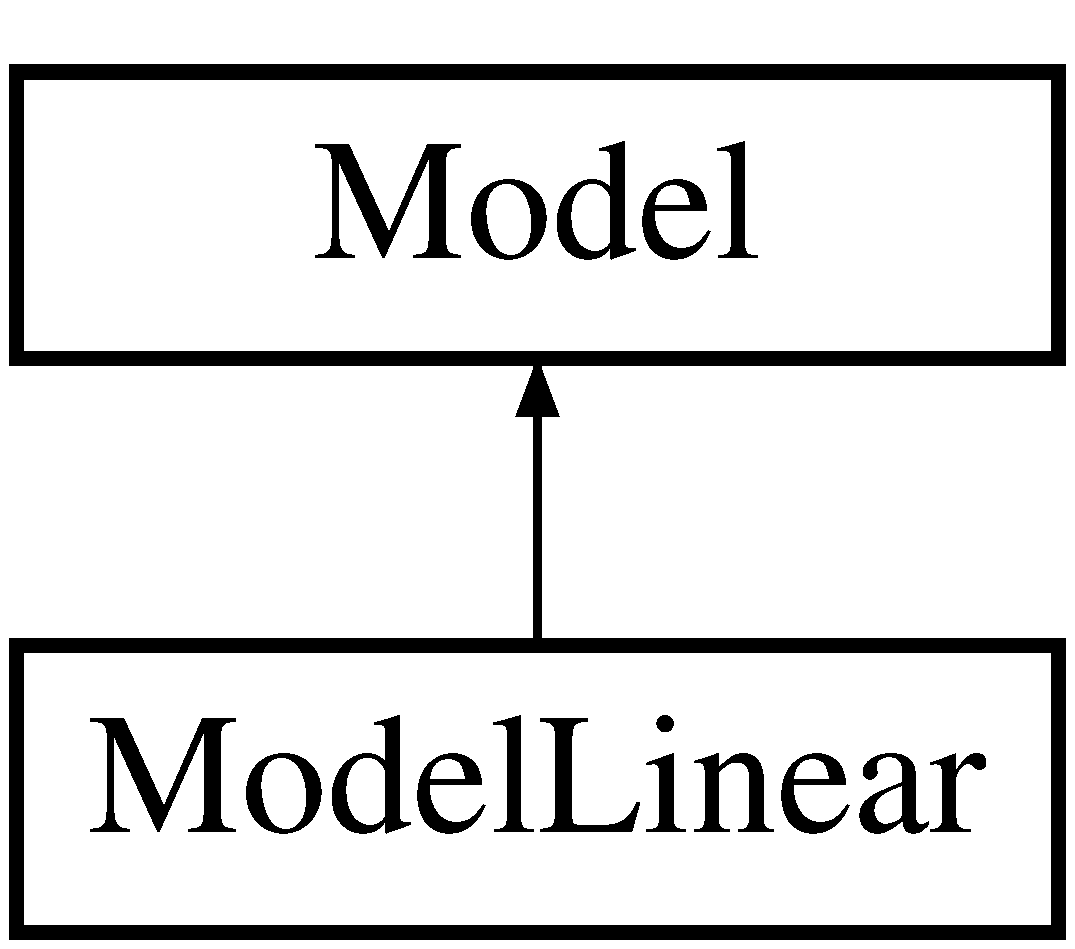
\includegraphics[height=2cm]{classModelLinear}
\end{center}
\end{figure}
\subsection*{Public Methods}
\begin{CompactItemize}
\item 
{\bf Model\-Linear} (string path)
\item 
virtual {\bf $\sim$Model\-Linear} ()
\item 
virtual {\bf MSLVector} {\bf State\-To\-Configuration} (const {\bf MSLVector} \&x)
\begin{CompactList}\small\item\em A method that converts a {\bf Model} {\rm (p.\,\pageref{classModel})} state in to a {\bf Geom} {\rm (p.\,\pageref{classGeom})} configuration.\item\end{CompactList}\item 
virtual {\bf MSLVector} {\bf Integrate} (const {\bf MSLVector} \&x, const {\bf MSLVector} \&u, const double \&h)
\begin{CompactList}\small\item\em Perform integration from state x, using input u, over time step h.\item\end{CompactList}\item 
virtual {\bf MSLVector} {\bf State\-Transition\-Equation} (const {\bf MSLVector} \&x, const {\bf MSLVector} \&u)
\begin{CompactList}\small\item\em The state transition equation, or equations of motion, xdot=f(x,u).\item\end{CompactList}\end{CompactItemize}
\subsection*{Public Attributes}
\begin{CompactItemize}
\item 
{\bf MSLMatrix} {\bf A}
\item 
{\bf MSLMatrix} {\bf B}
\end{CompactItemize}


\subsection{Detailed Description}
A linear systems model: xdot = Ax + Bu.



\subsection{Constructor \& Destructor Documentation}
\index{ModelLinear@{Model\-Linear}!ModelLinear@{ModelLinear}}
\index{ModelLinear@{ModelLinear}!ModelLinear@{Model\-Linear}}
\subsubsection{\setlength{\rightskip}{0pt plus 5cm}Model\-Linear::Model\-Linear (string {\em path} = \char`\"{}\char`\"{})}\label{classModelLinear_a0}


\index{ModelLinear@{Model\-Linear}!~ModelLinear@{$\sim$ModelLinear}}
\index{~ModelLinear@{$\sim$ModelLinear}!ModelLinear@{Model\-Linear}}
\subsubsection{\setlength{\rightskip}{0pt plus 5cm}Model\-Linear::$\sim$Model\-Linear ()\hspace{0.3cm}{\tt  [inline, virtual]}}\label{classModelLinear_a1}




\subsection{Member Function Documentation}
\index{ModelLinear@{Model\-Linear}!Integrate@{Integrate}}
\index{Integrate@{Integrate}!ModelLinear@{Model\-Linear}}
\subsubsection{\setlength{\rightskip}{0pt plus 5cm}{\bf MSLVector} Model\-Linear::Integrate (const {\bf MSLVector} \& {\em x}, const {\bf MSLVector} \& {\em u}, const double \& {\em h})\hspace{0.3cm}{\tt  [virtual]}}\label{classModelLinear_a3}


Perform integration from state x, using input u, over time step h.



Reimplemented from {\bf Model} {\rm (p.\,\pageref{classModel_a5})}.\index{ModelLinear@{Model\-Linear}!StateToConfiguration@{StateToConfiguration}}
\index{StateToConfiguration@{StateToConfiguration}!ModelLinear@{Model\-Linear}}
\subsubsection{\setlength{\rightskip}{0pt plus 5cm}{\bf MSLVector} Model\-Linear::State\-To\-Configuration (const {\bf MSLVector} \& {\em x})\hspace{0.3cm}{\tt  [virtual]}}\label{classModelLinear_a2}


A method that converts a {\bf Model} {\rm (p.\,\pageref{classModel})} state in to a {\bf Geom} {\rm (p.\,\pageref{classGeom})} configuration.



Reimplemented from {\bf Model} {\rm (p.\,\pageref{classModel_a8})}.\index{ModelLinear@{Model\-Linear}!StateTransitionEquation@{StateTransitionEquation}}
\index{StateTransitionEquation@{StateTransitionEquation}!ModelLinear@{Model\-Linear}}
\subsubsection{\setlength{\rightskip}{0pt plus 5cm}{\bf MSLVector} Model\-Linear::State\-Transition\-Equation (const {\bf MSLVector} \& {\em x}, const {\bf MSLVector} \& {\em u})\hspace{0.3cm}{\tt  [virtual]}}\label{classModelLinear_a4}


The state transition equation, or equations of motion, xdot=f(x,u).



Reimplemented from {\bf Model} {\rm (p.\,\pageref{classModel_a3})}.

\subsection{Member Data Documentation}
\index{ModelLinear@{Model\-Linear}!A@{A}}
\index{A@{A}!ModelLinear@{Model\-Linear}}
\subsubsection{\setlength{\rightskip}{0pt plus 5cm}{\bf MSLMatrix} Model\-Linear::A}\label{classModelLinear_m0}


\index{ModelLinear@{Model\-Linear}!B@{B}}
\index{B@{B}!ModelLinear@{Model\-Linear}}
\subsubsection{\setlength{\rightskip}{0pt plus 5cm}{\bf MSLMatrix} Model\-Linear::B}\label{classModelLinear_m1}




The documentation for this class was generated from the following files:\begin{CompactItemize}
\item 
{\bf modelmisc.h}\item 
{\bf modelmisc.C}\end{CompactItemize}
